\documentclass{article}\usepackage[]{graphicx}\usepackage[]{color}
% maxwidth is the original width if it is less than linewidth
% otherwise use linewidth (to make sure the graphics do not exceed the margin)
\makeatletter
\def\maxwidth{ %
  \ifdim\Gin@nat@width>\linewidth
    \linewidth
  \else
    \Gin@nat@width
  \fi
}
\makeatother

\definecolor{fgcolor}{rgb}{0.345, 0.345, 0.345}
\newcommand{\hlnum}[1]{\textcolor[rgb]{0.686,0.059,0.569}{#1}}%
\newcommand{\hlstr}[1]{\textcolor[rgb]{0.192,0.494,0.8}{#1}}%
\newcommand{\hlcom}[1]{\textcolor[rgb]{0.678,0.584,0.686}{\textit{#1}}}%
\newcommand{\hlopt}[1]{\textcolor[rgb]{0,0,0}{#1}}%
\newcommand{\hlstd}[1]{\textcolor[rgb]{0.345,0.345,0.345}{#1}}%
\newcommand{\hlkwa}[1]{\textcolor[rgb]{0.161,0.373,0.58}{\textbf{#1}}}%
\newcommand{\hlkwb}[1]{\textcolor[rgb]{0.69,0.353,0.396}{#1}}%
\newcommand{\hlkwc}[1]{\textcolor[rgb]{0.333,0.667,0.333}{#1}}%
\newcommand{\hlkwd}[1]{\textcolor[rgb]{0.737,0.353,0.396}{\textbf{#1}}}%
\let\hlipl\hlkwb

\usepackage{framed}
\makeatletter
\newenvironment{kframe}{%
 \def\at@end@of@kframe{}%
 \ifinner\ifhmode%
  \def\at@end@of@kframe{\end{minipage}}%
  \begin{minipage}{\columnwidth}%
 \fi\fi%
 \def\FrameCommand##1{\hskip\@totalleftmargin \hskip-\fboxsep
 \colorbox{shadecolor}{##1}\hskip-\fboxsep
     % There is no \\@totalrightmargin, so:
     \hskip-\linewidth \hskip-\@totalleftmargin \hskip\columnwidth}%
 \MakeFramed {\advance\hsize-\width
   \@totalleftmargin\z@ \linewidth\hsize
   \@setminipage}}%
 {\par\unskip\endMakeFramed%
 \at@end@of@kframe}
\makeatother

\definecolor{shadecolor}{rgb}{.97, .97, .97}
\definecolor{messagecolor}{rgb}{0, 0, 0}
\definecolor{warningcolor}{rgb}{1, 0, 1}
\definecolor{errorcolor}{rgb}{1, 0, 0}
\newenvironment{knitrout}{}{} % an empty environment to be redefined in TeX

\usepackage{alltt}

\usepackage{float}
\usepackage{amsfonts}
\usepackage{amsmath}
\usepackage{amssymb}
\usepackage{amsthm}
\usepackage{bm}
\usepackage{comment}

% Set the margins on the page to not be so large
\addtolength{\oddsidemargin}{-.875in}
\addtolength{\evensidemargin}{-.875in}
\addtolength{\textwidth}{1.75in}
\addtolength{\topmargin}{-.875in}
\addtolength{\textheight}{1.75in}

% Take off page numbering
\pagenumbering{gobble}
\IfFileExists{upquote.sty}{\usepackage{upquote}}{}
\begin{document}

\title{%
  7.1.1 - R: Principal Component Regression, Quantile Regression \\
  \smallskip
  \large Stat 5100: Dr. Bean
}
\date{}

\maketitle

\section*{Principal Components}

\textbf{Example:} Baseball dataset (we have seen this one quite a bit!)

\begin{knitrout}
\definecolor{shadecolor}{rgb}{0.969, 0.969, 0.969}\color{fgcolor}\begin{kframe}
\begin{alltt}
\hlkwd{library}\hlstd{(stat5100)}
\hlkwd{data}\hlstd{(baseball)}

\hlcom{# Look at multicollinearity in the baseball dataset}
\hlstd{baseball_lm} \hlkwb{<-} \hlkwd{lm}\hlstd{(logSalary} \hlopt{~} \hlstd{nAtBat} \hlopt{+} \hlstd{nHits} \hlopt{+} \hlstd{nHome} \hlopt{+} \hlstd{nRuns} \hlopt{+} \hlstd{nRBI} \hlopt{+} \hlstd{nBB} \hlopt{+}
                    \hlstd{YrMajor} \hlopt{+} \hlstd{CrAtBat} \hlopt{+} \hlstd{CrHits} \hlopt{+} \hlstd{CrHome} \hlopt{+} \hlstd{CrRuns} \hlopt{+} \hlstd{CrRbi} \hlopt{+}
                    \hlstd{CrBB} \hlopt{+} \hlstd{nOuts} \hlopt{+} \hlstd{nAssts} \hlopt{+} \hlstd{nError,} \hlkwc{data} \hlstd{= baseball)}
\hlstd{olsrr}\hlopt{::}\hlkwd{ols_vif_tol}\hlstd{(baseball_lm)}
\end{alltt}
\begin{verbatim}
##    Variables   Tolerance        VIF
## 1     nAtBat 0.046562403  21.476555
## 2      nHits 0.035153418  28.446736
## 3      nHome 0.129349044   7.731020
## 4      nRuns 0.068765678  14.542138
## 5       nRBI 0.087218325  11.465480
## 6        nBB 0.251956556   3.968938
## 7    YrMajor 0.108262158   9.236838
## 8    CrAtBat 0.004002379 249.851404
## 9     CrHits 0.002011778 497.072822
## 10    CrHome 0.019972282  50.069392
## 11    CrRuns 0.006210431 161.019424
## 12     CrRbi 0.007421451 134.744542
## 13      CrBB 0.048834939  20.477142
## 14     nOuts 0.795937680   1.256380
## 15    nAssts 0.368119153   2.716512
## 16    nError 0.455458468   2.195590
\end{verbatim}
\end{kframe}
\end{knitrout}

\subsubsection*{Consider using principal components}

\begin{knitrout}
\definecolor{shadecolor}{rgb}{0.969, 0.969, 0.969}\color{fgcolor}\begin{kframe}
\begin{alltt}
\hlcom{# Extract the principal components of the baseball dataset}
\hlstd{X} \hlkwb{<-} \hlkwd{subset}\hlstd{(baseball,} \hlkwc{select} \hlstd{=} \hlkwd{c}\hlstd{(}\hlstr{"nAtBat"}\hlstd{,} \hlstr{"nHits"}\hlstd{,} \hlstr{"nHome"}\hlstd{,} \hlstr{"nRuns"}\hlstd{,} \hlstr{"nRBI"}\hlstd{,}
                                 \hlstr{"nBB"}\hlstd{,} \hlstr{"YrMajor"}\hlstd{,} \hlstr{"CrAtBat"}\hlstd{,} \hlstr{"CrHits"}\hlstd{,} \hlstr{"CrHome"}\hlstd{,}
                                 \hlstr{"CrRuns"}\hlstd{,} \hlstr{"CrRbi"}\hlstd{,} \hlstr{"CrBB"}\hlstd{,} \hlstr{"nOuts"}\hlstd{,} \hlstr{"nAssts"}\hlstd{,}
                                 \hlstr{"nError"}\hlstd{))}

\hlcom{# We standardize our data so that the portions of "explained variation" are not}
\hlcom{# sensitive to individual variable scale.}
\hlstd{X} \hlkwb{<-} \hlkwd{scale}\hlstd{(X)}

\hlcom{# This function will get you the principal components of your data matrix X}
\hlstd{X_pc} \hlkwb{<-} \hlkwd{prcomp}\hlstd{(X)}

\hlcom{# To see all 16 principal components, you can directly output the X_pc object.}
\hlcom{# However, this will get really messy so don't worry too much about this}
\hlcom{# output. We mostly care about the first few principal components anyway.}
\hlstd{X_pc}
\end{alltt}
\begin{verbatim}
## Standard deviations (1, .., p=16):
##  [1] 2.67713151 2.07308677 1.28860973 0.92409050 0.82764973 0.71528498
##  [7] 0.50395676 0.42817178 0.35992487 0.30830228 0.24852168 0.22900605
## [13] 0.16530173 0.12170647 0.06857458 0.03517156
## 
## Rotation (n x k) = (16 x 16):
##                  PC1        PC2         PC3           PC4           PC5
## nAtBat   0.194632762 -0.3848602 -0.05821051  0.0528472981 -0.1024266929
## nHits    0.190051488 -0.3786146 -0.03860149  0.0714295481 -0.1525168732
## nHome    0.203519373 -0.2369245  0.34019459  0.1463279498  0.5058998723
## nRuns    0.189950679 -0.3772638  0.06692317  0.1565906990 -0.2163922848
## nRBI     0.233485481 -0.3139654  0.17448967  0.0840865127  0.3028003293
## nBB      0.207015079 -0.2452606  0.06951211  0.0024775582 -0.5426914501
## YrMajor  0.285640403  0.2603009 -0.09246630 -0.0398197197  0.0001121828
## CrAtBat  0.333086248  0.1881212 -0.12562043 -0.0372534708 -0.0274971057
## CrHits   0.333439379  0.1775303 -0.12338161 -0.0446229161 -0.0427622485
## CrHome   0.320242184  0.1218643  0.11115310  0.0589002322  0.2760028790
## CrRuns   0.341921106  0.1655446 -0.08899579  0.0105678949 -0.0758996071
## CrRbi    0.343103280  0.1642071 -0.01441149 -0.0210341359  0.1328582618
## CrBB     0.320946272  0.1796460 -0.05986120 -0.0008438691 -0.1744154829
## nOuts    0.084464959 -0.1714051  0.15181459 -0.9548574775  0.0156331012
## nAssts   0.008005724 -0.1860940 -0.65572378  0.0294239528  0.0410271729
## nError  -0.004220569 -0.2262277 -0.56832264 -0.1322441492  0.3778389483
##                  PC6          PC7          PC8         PC9         PC10
## nAtBat  -0.284596589  0.001662044 -0.179778166  0.11897679  0.075554512
## nHits   -0.394034569  0.026601804 -0.144598334  0.08532095 -0.017798355
## nHome    0.215119585 -0.107931196  0.375147634 -0.32302858  0.098307597
## nRuns   -0.114011922  0.138021924 -0.017323225 -0.47803071  0.333872534
## nRBI    -0.024618272 -0.106075830  0.194902333  0.44863472 -0.413056034
## nBB      0.631883065  0.072884957  0.085231276  0.31231296 -0.002799702
## YrMajor -0.148894876 -0.018198069  0.442545336  0.35670668  0.672218705
## CrAtBat -0.153360981  0.056440704  0.123152978 -0.03269411 -0.143514748
## CrHits  -0.201340974  0.093766410  0.108009464 -0.03452201 -0.268355707
## CrHome   0.244057499 -0.131170044 -0.666811335  0.05327312  0.275254186
## CrRuns  -0.079355223  0.083711382  0.016431236 -0.25848725 -0.219481860
## CrRbi    0.004120958 -0.026170699 -0.285253023  0.15399932 -0.042270828
## CrBB     0.291356490 -0.011625910  0.090072946 -0.32492627 -0.168131226
## nOuts   -0.024460243 -0.123255967 -0.009238466 -0.09587398  0.035701024
## nAssts   0.116668965 -0.702628391  0.057429867 -0.09229836  0.011591606
## nError   0.231040700  0.637028488 -0.005623412  0.02708960  0.048229516
##                 PC11         PC12         PC13        PC14         PC15
## nAtBat  -0.059299021  0.606954871 -0.515354079  0.09159705 -0.126379177
## nHits   -0.225552025  0.053853770  0.725130632 -0.10804571  0.071796485
## nHome    0.186070251  0.333914734  0.210785731  0.04738002 -0.055261821
## nRuns    0.095608558 -0.541980891 -0.214725535  0.13971644  0.036052625
## nRBI    -0.222619669 -0.411615022 -0.250002874 -0.09935857  0.062445908
## nBB      0.267431044  0.071021353  0.095709357 -0.04653579  0.009062175
## YrMajor -0.151353549 -0.046689104 -0.006053483 -0.10482943 -0.081207508
## CrAtBat  0.231925832  0.085913959 -0.085733669  0.20560043  0.714547626
## CrHits   0.316668866  0.017926738  0.115434077  0.06143162 -0.045866151
## CrHome  -0.028952446 -0.024571161 -0.005716373 -0.26823670  0.281744440
## CrRuns   0.131837200 -0.008358208 -0.112663559 -0.67377779 -0.345141168
## CrRbi    0.165044985 -0.149424718  0.107626721  0.56846377 -0.502602976
## CrBB    -0.739889851  0.101161434 -0.016201822  0.19803174 -0.001737193
## nOuts   -0.006224165 -0.037906494 -0.007907441 -0.02334402  0.003117727
## nAssts   0.092505349 -0.066273274  0.017839679 -0.00883109 -0.011644225
## nError  -0.047949208 -0.006766120  0.027052974 -0.01342598  0.001089662
##                 PC16
## nAtBat  -0.047790523
## nHits    0.098917950
## nHome    0.029051734
## nRuns   -0.060174027
## nRBI    -0.026685140
## nBB      0.016386201
## YrMajor -0.018552281
## CrAtBat  0.388370291
## CrHits  -0.764363972
## CrHome  -0.194362505
## CrRuns   0.331792966
## CrRbi    0.304185822
## CrBB    -0.081124274
## nOuts    0.002488037
## nAssts  -0.007155282
## nError   0.005189008
\end{verbatim}
\begin{alltt}
\hlcom{# If we want a more concise summary, we can use the summary function:}
\hlkwd{summary}\hlstd{(X_pc)}
\end{alltt}
\begin{verbatim}
## Importance of components:
##                           PC1    PC2    PC3     PC4     PC5     PC6     PC7
## Standard deviation     2.6771 2.0731 1.2886 0.92409 0.82765 0.71528 0.50396
## Proportion of Variance 0.4479 0.2686 0.1038 0.05337 0.04281 0.03198 0.01587
## Cumulative Proportion  0.4479 0.7166 0.8203 0.87370 0.91651 0.94849 0.96436
##                            PC8    PC9    PC10    PC11    PC12    PC13    PC14
## Standard deviation     0.42817 0.3599 0.30830 0.24852 0.22901 0.16530 0.12171
## Proportion of Variance 0.01146 0.0081 0.00594 0.00386 0.00328 0.00171 0.00093
## Cumulative Proportion  0.97582 0.9839 0.98986 0.99372 0.99700 0.99870 0.99963
##                           PC15    PC16
## Standard deviation     0.06857 0.03517
## Proportion of Variance 0.00029 0.00008
## Cumulative Proportion  0.99992 1.00000
\end{verbatim}
\end{kframe}
\end{knitrout}

Note that the first principal component represents 97.5\% percent of the total variation in the dataset (this comes from the summary output). This tells us that most likely we can discard all the principal components past the first 2 or so.

\begin{knitrout}
\definecolor{shadecolor}{rgb}{0.969, 0.969, 0.969}\color{fgcolor}\begin{kframe}
\begin{alltt}
\hlcom{# Also show a scree plot. A scree plot is a plot that contains the relative}
\hlcom{# "importance" of the principal components on the y-axis and the number of the}
\hlcom{# principal component on the x-axis.}
\hlkwd{screeplot}\hlstd{(X_pc,} \hlkwc{type} \hlstd{=} \hlstr{"lines"}\hlstd{)}
\end{alltt}
\end{kframe}

{\centering 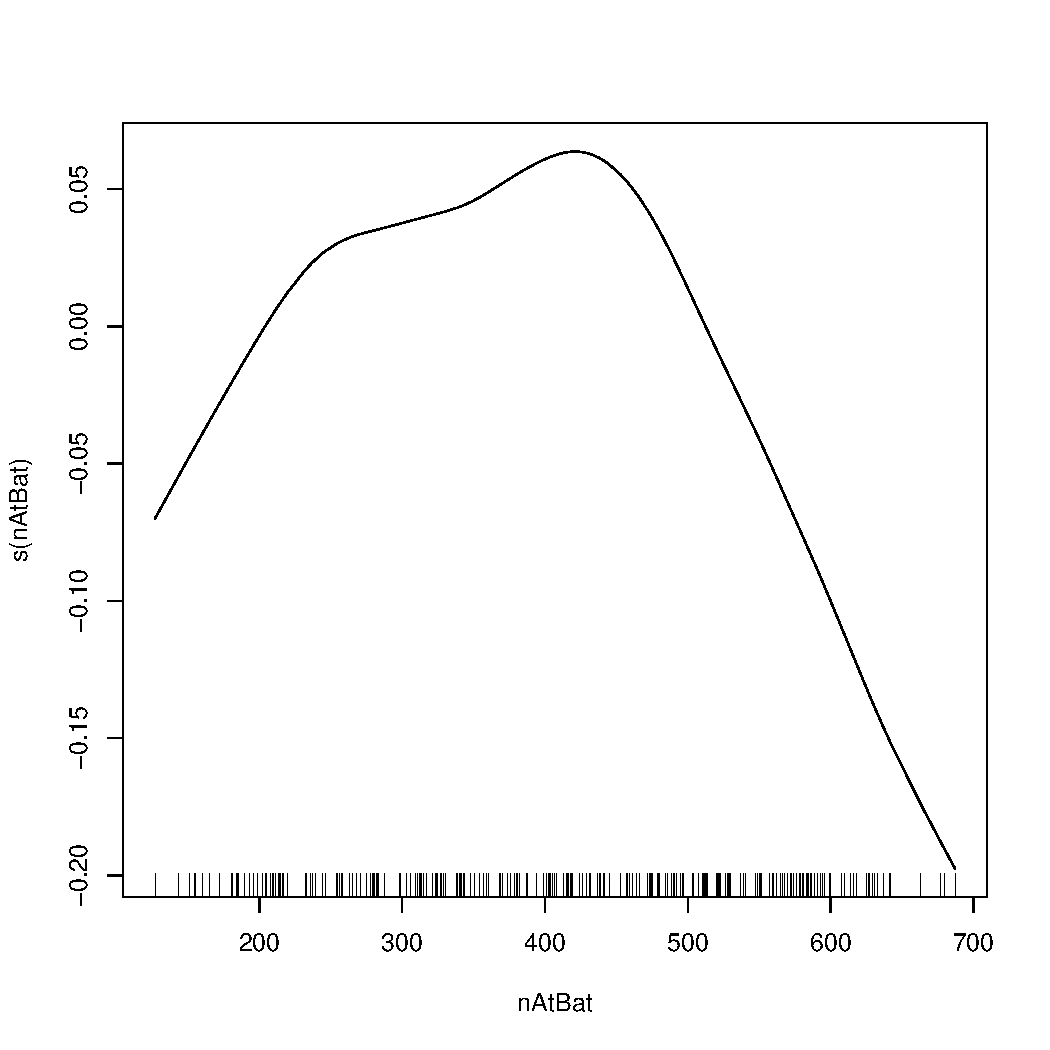
\includegraphics[width=0.6\textwidth]{figure/unnamed-chunk-3-1} 

}



\end{knitrout}

Now, let's fit a regression model with the principal components. Note that from the above summary, the first 6 principal components explain 95\% of the variation in our data matrix. Thus, we will use the first 6 principal components to fit a regression model.

Because each PC (principal component) is simply a linear combination of our predictor variables, let's calculate what each PC is for each of the observations in our dataset.

\begin{knitrout}
\definecolor{shadecolor}{rgb}{0.969, 0.969, 0.969}\color{fgcolor}\begin{kframe}
\begin{alltt}
\hlcom{# Let's say you wanted to grab the 3rd principal component. Here is how you do}
\hlcom{# it if you got the principal components from the prcomp() function:}
\hlstd{X_pc}\hlopt{$}\hlstd{rotation[,} \hlnum{3}\hlstd{]}
\end{alltt}
\begin{verbatim}
##      nAtBat       nHits       nHome       nRuns        nRBI         nBB 
## -0.05821051 -0.03860149  0.34019459  0.06692317  0.17448967  0.06951211 
##     YrMajor     CrAtBat      CrHits      CrHome      CrRuns       CrRbi 
## -0.09246630 -0.12562043 -0.12338161  0.11115310 -0.08899579 -0.01441149 
##        CrBB       nOuts      nAssts      nError 
## -0.05986120  0.15181459 -0.65572378 -0.56832264
\end{verbatim}
\end{kframe}
\end{knitrout}


With the above in mind, we can create our PC matrix for all observations in our dataset. To do this for a particular observation, we need the dot product between the principal component and the observation's recorded values (this is how the linear combination is done). Recall that in matrix multiplication with $A \in \mathbb{R}^{p \times n}$ and $B \in \mathbb{R}^{n \times d}$, the multiplication $AB$ calculates the dot products between the rows of $A$ and the columns of $B$. Because we want the dot product between our observations (columns of the matrix $X$) and the principal components, we can efficiently do this with the matrix multiplication
\[\tilde{X} = X P\]
In this particular example, $X \in \mathbb{R}^{322 \times 16}$ and $P \in \mathbb{R}^{16 \times 6}$ because we have 322 observations, 16 original variables, and 6 principal components we wish to use. In the matrix $P$ we will have the principal components along the columns of the matrix.

\begin{knitrout}
\definecolor{shadecolor}{rgb}{0.969, 0.969, 0.969}\color{fgcolor}\begin{kframe}
\begin{alltt}
\hlcom{# The data of just principal components will just be called "Xtilde"}
\hlstd{Xtilde} \hlkwb{=} \hlstd{X} \hlopt \hlstd{X_pc}\hlopt{$}\hlstd{rotation[,} \hlnum{1}\hlopt{:}\hlnum{6}\hlstd{]}

\hlstd{Xtilde} \hlkwb{<-} \hlkwd{as.data.frame}\hlstd{(Xtilde)}
\hlstd{baseball_pc_augmented} \hlkwb{=} \hlkwd{cbind}\hlstd{(}\hlkwc{logSalary} \hlstd{= baseball}\hlopt{$}\hlstd{logSalary, Xtilde)}

\hlcom{# Now we can fit a linear model with the principal components}
\hlstd{baseball_pc_lm} \hlkwb{<-} \hlkwd{lm}\hlstd{(logSalary} \hlopt{~} \hlstd{.,} \hlkwc{data} \hlstd{= baseball_pc_augmented)}

\hlcom{# Check out the summary of the linear model}
\hlkwd{summary}\hlstd{(baseball_pc_lm)}
\end{alltt}
\begin{verbatim}
## 
## Call:
## lm(formula = logSalary ~ ., data = baseball_pc_augmented)
## 
## Residuals:
##      Min       1Q   Median       3Q      Max 
## -2.05301 -0.44195  0.07629  0.44273  1.20518 
## 
## Coefficients:
##             Estimate Std. Error t value Pr(>|t|)    
## (Intercept)  5.90090    0.03683 160.218  < 2e-16 ***
## PC1          0.24502    0.01376  17.808  < 2e-16 ***
## PC2         -0.03595    0.01798  -1.999  0.04666 *  
## PC3         -0.01165    0.02672  -0.436  0.66327    
## PC4         -0.04607    0.03914  -1.177  0.24030    
## PC5         -0.12989    0.04327  -3.002  0.00295 ** 
## PC6         -0.13415    0.04953  -2.708  0.00722 ** 
## ---
## Signif. codes:  0 '***' 0.001 '**' 0.01 '*' 0.05 '.' 0.1 ' ' 1
## 
## Residual standard error: 0.5897 on 256 degrees of freedom
##   (59 observations deleted due to missingness)
## Multiple R-squared:  0.5703,	Adjusted R-squared:  0.5602 
## F-statistic: 56.63 on 6 and 256 DF,  p-value: < 2.2e-16
\end{verbatim}
\end{kframe}
\end{knitrout}

Using the above, we can use the linear regression model in the same way that we normally use our linear regression models. Just keep in mind that we are using new predictor variables that are principal components, and we obtain them by standardizing our data and then transforming them into the principal component by taking the dot product between the principal component and the observation's data to get the correct linear combination.

Principal components are a great way to capture the main trends and variability in your model while reducing the number of required dimensions to represent your data. Using principal components can also help eliminate multicollinearity.

Note also that there are packages such as ``pls'' in R that allow you to do principal components regression more easily. I chose to take this more manual approach with matrix multiplication for an insight into what principal components regression is really doing.

\bigskip
\hrule
\bigskip

\section*{Quantile Regression}

To do quantile regression in R, we can use the ``quantreg'' package. To fit a different regression for various quantiles, we can pass in a vector for the $\tau$ (tau) parameter.

\begin{knitrout}
\definecolor{shadecolor}{rgb}{0.969, 0.969, 0.969}\color{fgcolor}\begin{kframe}
\begin{alltt}
\hlstd{qr_baseball} \hlkwb{<-} \hlstd{quantreg}\hlopt{::}\hlkwd{rq}\hlstd{(Salary} \hlopt{~} \hlstd{nAtBat} \hlopt{+} \hlstd{nHits} \hlopt{+} \hlstd{nHome} \hlopt{+} \hlstd{nRuns} \hlopt{+} \hlstd{nRBI} \hlopt{+} \hlstd{nBB} \hlopt{+} \hlstd{YrMajor} \hlopt{+}
                            \hlstd{CrAtBat} \hlopt{+} \hlstd{CrHits} \hlopt{+} \hlstd{CrHome} \hlopt{+} \hlstd{CrRbi} \hlopt{+} \hlstd{CrBB} \hlopt{+} \hlstd{nOuts} \hlopt{+}
                            \hlstd{nAssts} \hlopt{+} \hlstd{nError,} \hlkwc{tau} \hlstd{=} \hlkwd{c}\hlstd{(}\hlnum{0.1}\hlstd{,} \hlnum{0.5}\hlstd{,} \hlnum{0.9}\hlstd{),} \hlkwc{data} \hlstd{= baseball)}
\end{alltt}
\end{kframe}
\end{knitrout}

In the below, note that we have different estimated regression functions depending on the different quantiles.

\begin{knitrout}
\definecolor{shadecolor}{rgb}{0.969, 0.969, 0.969}\color{fgcolor}\begin{kframe}
\begin{alltt}
\hlkwd{summary}\hlstd{(qr_baseball)}
\end{alltt}
\begin{verbatim}
## 
## Call: quantreg::rq(formula = Salary ~ nAtBat + nHits + nHome + nRuns + 
##     nRBI + nBB + YrMajor + CrAtBat + CrHits + CrHome + CrRbi + 
##     CrBB + nOuts + nAssts + nError, tau = c(0.1, 0.5, 0.9), data = baseball)
## 
## tau: [1] 0.1
## 
## Coefficients:
##             coefficients lower bd   upper bd  
## (Intercept)   -8.94681   -107.76066   18.49711
## nAtBat        -0.51824     -1.41573   -0.09214
## nHits          1.26452      0.12059    4.25142
## nHome          0.60066     -4.55762    5.84193
## nRuns          1.73852     -2.04437    3.49574
## nRBI           0.16803     -2.45665    2.57170
## nBB            1.39984      0.26270    3.80735
## YrMajor       15.21422     -2.99852   21.73511
## CrAtBat       -0.17598     -0.26956    0.08859
## CrHits         0.62361      0.44394    1.38512
## CrHome        -0.34961     -0.67154    2.26702
## CrRbi          0.19413     -0.55298    0.21587
## CrBB           0.00019     -0.62606    0.17172
## nOuts         -0.01192     -0.03050    0.02078
## nAssts         0.10020      0.02885    0.44811
## nError         0.01154     -8.60334    1.04383
## 
## Call: quantreg::rq(formula = Salary ~ nAtBat + nHits + nHome + nRuns + 
##     nRBI + nBB + YrMajor + CrAtBat + CrHits + CrHome + CrRbi + 
##     CrBB + nOuts + nAssts + nError, tau = c(0.1, 0.5, 0.9), data = baseball)
## 
## tau: [1] 0.5
## 
## Coefficients:
##             coefficients lower bd   upper bd  
## (Intercept)  -46.90574   -153.24381   27.47963
## nAtBat        -1.33327     -2.50219   -0.01376
## nHits          6.54961      1.57072   11.49926
## nHome         -1.21370    -13.77272    6.61687
## nRuns         -1.80900     -5.42341    3.29437
## nRBI          -1.18111     -4.45098    5.80451
## nBB            4.71468     -0.06785    6.96886
## YrMajor        9.53819     -6.12636   34.94063
## CrAtBat       -0.15957     -0.42149    0.15568
## CrHits         1.06059     -0.62519    1.88644
## CrHome         3.77373     -1.91154    8.54287
## CrRbi         -1.00979     -2.75024    1.40345
## CrBB          -0.21883     -0.97622    0.30700
## nOuts          0.27225      0.02250    0.50623
## nAssts         0.20481     -0.30142    0.55061
## nError        -2.77023     -8.13893    5.63963
## 
## Call: quantreg::rq(formula = Salary ~ nAtBat + nHits + nHome + nRuns + 
##     nRBI + nBB + YrMajor + CrAtBat + CrHits + CrHome + CrRbi + 
##     CrBB + nOuts + nAssts + nError, tau = c(0.1, 0.5, 0.9), data = baseball)
## 
## tau: [1] 0.9
## 
## Coefficients:
##             coefficients lower bd   upper bd  
## (Intercept)  -87.68624   -154.75738  229.93587
## nAtBat        -0.84463     -2.61028    0.64170
## nHits          2.86591     -3.74737    9.76884
## nHome          0.00721    -22.16688   17.16975
## nRuns          0.86999     -4.66778    7.21654
## nRBI           3.50664      0.49331    9.75059
## nBB            1.96045     -1.71872    9.12183
## YrMajor       36.17809    -21.47820   52.19125
## CrAtBat       -0.60494     -1.05634    0.46398
## CrHits         2.77600     -0.63185    4.24905
## CrHome         5.19422     -1.52798   11.45764
## CrRbi         -1.92070     -4.67270    1.07168
## CrBB           0.27451     -1.33273    1.52485
## nOuts          0.48872      0.13158    0.64450
## nAssts         0.15241     -0.32073    0.51382
## nError         3.36747     -7.80390   15.06840
\end{verbatim}
\end{kframe}
\end{knitrout}

Note also that in the quantreg package, there are functions such as ``rq.fit.lasso'' that allow you to to automatically perform variable selection via Lasso regression. This is done separately for each of the quantiles, so each quantile may end up with completely different variables! Note also that this function does require you to set your own $\lambda$ penalty parameter, so if you use this function make sure to test out a few values of $\lambda$ for best results.

\end{document}
